\begin{figure}[h!]
	\centering
	
	
	
	\tikzset{every picture/.style={line width=0.75pt}} %set default line width to 0.75pt        
	
	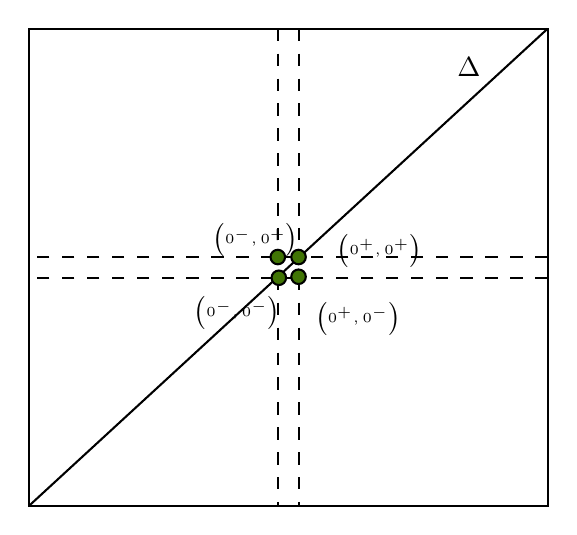
\begin{tikzpicture}[x=0.75pt,y=0.75pt,yscale=-1,xscale=1]
		%uncomment if require: \path (0,300); %set diagram left start at 0, and has height of 300
		
		%Shape: Rectangle [id:dp5193643571266664] 
		\draw   (150,20) -- (400,20) -- (400,250) -- (150,250) -- cycle ;
		%Straight Lines [id:da2432122097230004] 
		\draw [color={rgb, 255:red, 0; green, 0; blue, 0 }  ,draw opacity=1 ][line width=0.75]  [dash pattern={on 4.5pt off 4.5pt}]  (270,20) -- (270,250) ;
		%Straight Lines [id:da8789847469102436] 
		\draw [color={rgb, 255:red, 0; green, 0; blue, 0 }  ,draw opacity=1 ][line width=0.75]  [dash pattern={on 4.5pt off 4.5pt}]  (280,20) -- (280,250) ;
		%Straight Lines [id:da6533899359137522] 
		\draw [color={rgb, 255:red, 0; green, 0; blue, 0 }  ,draw opacity=1 ][line width=0.75]  [dash pattern={on 4.5pt off 4.5pt}]  (400,130) -- (150,130) ;
		%Straight Lines [id:da535776408423082] 
		\draw [color={rgb, 255:red, 0; green, 0; blue, 0 }  ,draw opacity=1 ][line width=0.75]  [dash pattern={on 4.5pt off 4.5pt}]  (400,140) -- (150,140) ;
		%Straight Lines [id:da5554446790214769] 
		\draw    (400,20) -- (150,250) ;
		%Shape: Circle [id:dp32546629561587426] 
		\draw  [fill={rgb, 255:red, 65; green, 117; blue, 5 }  ,fill opacity=1 ] (276.5,130) .. controls (276.5,128.07) and (278.07,126.5) .. (280,126.5) .. controls (281.93,126.5) and (283.5,128.07) .. (283.5,130) .. controls (283.5,131.93) and (281.93,133.5) .. (280,133.5) .. controls (278.07,133.5) and (276.5,131.93) .. (276.5,130) -- cycle ;
		%Shape: Circle [id:dp8202919592455564] 
		\draw  [fill={rgb, 255:red, 65; green, 117; blue, 5 }  ,fill opacity=1 ] (266.5,130) .. controls (266.5,128.07) and (268.07,126.5) .. (270,126.5) .. controls (271.93,126.5) and (273.5,128.07) .. (273.5,130) .. controls (273.5,131.93) and (271.93,133.5) .. (270,133.5) .. controls (268.07,133.5) and (266.5,131.93) .. (266.5,130) -- cycle ;
		%Shape: Circle [id:dp7704702433707692] 
		\draw  [fill={rgb, 255:red, 65; green, 117; blue, 5 }  ,fill opacity=1 ] (276.5,139.5) .. controls (276.5,137.57) and (278.07,136) .. (280,136) .. controls (281.93,136) and (283.5,137.57) .. (283.5,139.5) .. controls (283.5,141.43) and (281.93,143) .. (280,143) .. controls (278.07,143) and (276.5,141.43) .. (276.5,139.5) -- cycle ;
		%Shape: Circle [id:dp40492667019933914] 
		\draw  [fill={rgb, 255:red, 65; green, 117; blue, 5 }  ,fill opacity=1 ] (267,140) .. controls (267,138.07) and (268.57,136.5) .. (270.5,136.5) .. controls (272.43,136.5) and (274,138.07) .. (274,140) .. controls (274,141.93) and (272.43,143.5) .. (270.5,143.5) .. controls (268.57,143.5) and (267,141.93) .. (267,140) -- cycle ;
		
		% Text Node
		\draw (297,117.4) node [anchor=north west][inner sep=0.75pt]  [font=\tiny,color={rgb, 255:red, 0; green, 0; blue, 0 }  ,opacity=1 ]  {$\left( 0^{+} ,0^{+}\right)$};
		% Text Node
		\draw (286.5,150.4) node [anchor=north west][inner sep=0.75pt]  [font=\tiny,color={rgb, 255:red, 0; green, 0; blue, 0 }  ,opacity=1 ]  {$\left( 0^{+} ,0^{-}\right)$};
		% Text Node
		\draw (228,147.4) node [anchor=north west][inner sep=0.75pt]  [font=\tiny,color={rgb, 255:red, 0; green, 0; blue, 0 }  ,opacity=1 ]  {$\left( 0^{-} ,0^{-}\right)$};
		% Text Node
		\draw (237,112.4) node [anchor=north west][inner sep=0.75pt]  [font=\tiny,color={rgb, 255:red, 0; green, 0; blue, 0 }  ,opacity=1 ]  {$\left( 0^{-} ,0^{+}\right)$};
		% Text Node
		\draw (355,32.4) node [anchor=north west][inner sep=0.75pt]    {$\Delta $};
		
		
	\end{tikzpicture}
\end{figure}